The Standard Model (SM) of particle physics provides precise predictions for the properties and interactions of fundamental particles, which have been confirmed by numerous experiments since the inception of the model in the 1960’s. However, it is clear that the model is incomplete. The SM is unable to explain cosmological observations of the dominance of matter over antimatter,  the apparent dark-matter content of the Universe,  or explain the patterns seen in the interaction strengths of the particles.
Particle physicists have therefore been searching for ‘new physics’~\textemdash~the new particles and interactions that can explain the SM’s shortcomings. 

One method to search for new physics is to compare measurements of the properties of hadron decays, where hadrons are bound states of quarks, with their SM predictions. Measurable quantities can be predicted precisely  in the decays 
of a charged beauty hadron, \Bp, into a charged kaon, \Kp, and two charged leptons,~$\ell^{+}\ell^{-}$. The \Bp hadron contains a beauty antiquark, \bquarkbar, and the \Kp a strange antiquark, \squarkbar, such that at the quark level the decay involves a $\bquarkbar\to\squarkbar$ transition.
Quantum field theory allows such a process to be mediated by virtual particles that can have a physical mass larger than the mass difference between the initial- and final-state particles. In the SM description of such processes, these virtual particles include the electroweak-force carriers, the $\gamma$, $W^{\pm}$ and $Z^0$ bosons, and the top quark~(see Fig.~\ref{fig:feyn}, left). Such decays are highly suppressed~\cite{Glashow:1970gm} and the fraction of \Bp hadrons that decay into this final state (the branching fraction, \BR) is of the order of $10^{-6}$~\cite{PDG2020}.

\begin{figure}[b!]
   \begin{center}
   % FDs_RK_forPaper_withLQ
      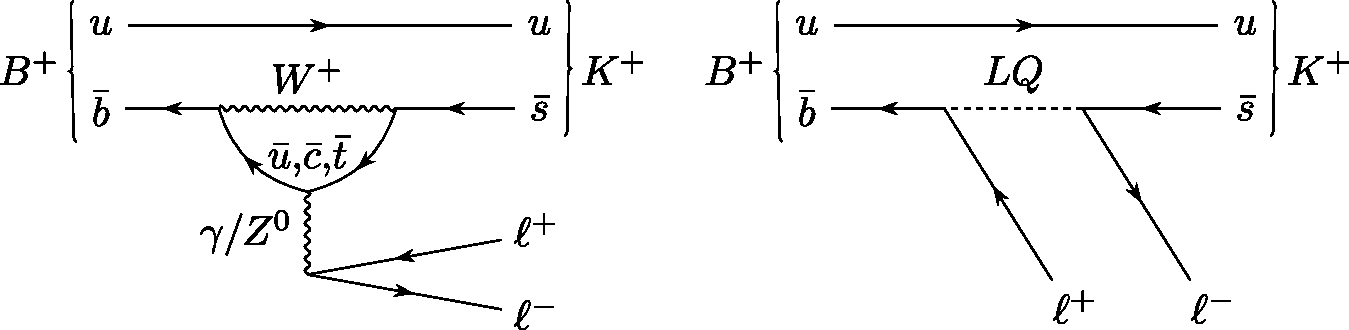
\includegraphics[width=0.96\linewidth]{figures/Fig1.pdf}
   \end{center}
   \vspace*{-0.5cm}
   \caption{
  Fundamental processes contributing to \BuKll decays in the SM and possible new physics models. A \Bp meson, consisting of \bquarkbar and \uquark quarks, decays into a \Kp, containing \squarkbar and \uquark quarks, and two charged leptons, $\ellp\ellm$. (Left) The SM contribution involves the electroweak bosons $\gamma,~W^+$ and $Z^0$. (Right) A possible new physics contribution to the decay with a hypothetical leptoquark ($LQ$) which, unlike the electroweak bosons, could have different interaction strengths with the different types of leptons.     
   }\label{fig:feyn}
\end{figure}

A distinctive feature of the SM is that the different leptons, electron ($\en$), muon ($\mun$) and tau ($\taum$),
 have the same interaction strengths. This is known as ‘lepton universality’. The only exception to this is due to the Higgs field, since the lepton-Higgs interaction strength gives rise to the differing lepton masses $m_{\tau}>m_{\mu}>m_e$. 
The suppression of $\bquarkbar \to \squarkbar$ transitions is understood in terms of the fundamental symmetries on which the SM is built. Conversely, lepton universality is an accidental symmetry of the SM, which is not a consequence of any axiom of the theory. Extensions to the SM that aim to address many of its shortfalls predict new virtual particles that could contribute to $\bquarkbar \to \squarkbar$ transitions~(see Fig.~\ref{fig:feyn}, right) and could have nonuniversal interactions, hence giving branching fractions of \BuKll
 decays with different leptons that differ from the SM predictions. Whenever a process is specified in this article, the inclusion of the charge-conjugate mode is implied.


Calculation of the SM predictions for the branching fractions of \BuKmm and \BuKee decays is complicated by the strong nuclear force that binds together the quarks into hadrons, as described by quantum chromodynamics (QCD). The large interaction strengths preclude predictions of QCD effects with the perturbation techniques used to compute the electroweak force amplitudes and only approximate  calculations are presently possible. However, the strong force does not  couple directly to leptons and hence its effect on the \BuKmm and \BuKee decays is identical. The ratio between the branching fractions of these decays is therefore predicted with $\mathcal{O}(1\%)$ precision~\cite{Descotes-Genon:2015uva,Bobeth:2007,Bordone:2016gaq,EOS,Straub:2018kue,Isidori:2020acz}. 
Due to the small masses of both electrons and muons compared to that of \bquark quarks, this ratio is predicted to be close to unity, 
except where the value of the dilepton invariant mass-squared (\qsq) significantly restricts the phase space available to form the two leptons.
Similar considerations apply to decays with other $B$ hadrons, \BuzHmm and \BuzHee, where $B=\Bu$, \Bz, \Bs or \Lb; and $H$ can be \eg an excited kaon, $\Kstarz$, or a combination of particles such as a proton and charged kaon, $p\Km$. 
The ratio of branching fractions, \RH~\cite{Hiller:2003js, Wang:2003je}, is defined in the dilepton mass-squared range $q^{2}_{\rm min} < \qsq < q^{2}_{\rm max}$ as
\begin{equation}
\label{eq:rh}
\RH \equiv  \dfrac{\displaystyle\int_{q^2_\mathrm{min}}^{q^2_{\rm max}} \dfrac{\deriv\BF(\BuzHmm)}{\deriv\qsq} \deriv\qsq}{\displaystyle\int_{q^2_{\rm min}}^{q^2_{\rm max}} \dfrac{\deriv\BF(\BuzHee)}{\deriv\qsq} \deriv\qsq} ~.
\end{equation}
\noindent 
For decays with $H\!=\!\Kp$ and $H\!=\!\Kstarz$ such ratios, denoted \RK and \RKstar, respectively, have previously been measured in similar regions of \qsq~\cite{LHCb-PAPER-2019-009, LHCb-PAPER-2017-013}.
For \RK the measurements are in the region $1.1 < \qsq < 6.0 \gevgevcccc$, whereas for \RKstar the regions are \mbox{$0.045 < \qsq < 1.1 \gevgevcccc$} and $1.1 < \qsq < 6.0 \gevgevcccc$. These ratios have been determined to be 
$2.1$--$2.5$~standard deviations below their respective SM expectations~\cite{Descotes-Genon:2015uva,Bobeth:2007,Bordone:2016gaq,Capdevila:2016ivx,Capdevila:2017ert,Serra:2016ivr,EOS,Straub:2015ica,Straub:2018kue,Altmannshofer:2017fio,Jager:2014rwa}. 
The analogous ratio has also been measured for \Lb decays with $H=p\Km$ and is compatible with unity at the level of one standard deviation~\cite{LHCb-PAPER-2019-040}.

These decays all proceed via
 the same \btosbar quark transition and the results have therefore further increased interest in measurements of angular observables~\cite{LHCb-PAPER-2020-041,LHCb-PAPER-2020-002,LHCb-PAPER-2015-051,Aaboud:2018krd,Aubert:2006vb,Lees:2015ymt,Wei:2009zv,Wehle:2016yoi,Aaltonen:2011ja,Khachatryan:2015isa,Sirunyan:2017dhj} and branching fractions~\cite{LHCb-PAPER-2016-012, LHCb-PAPER-2015-023, LHCb-PAPER-2014-006, LHCb-PAPER-2015-009} of decays mediated by \btosmumubar transitions. Such decays also exhibit some tension with the SM predictions but the extent of residual QCD effects is still the subject of debate~\cite{Jager:2014rwa, Descotes-Genon:2015uva,Lyon:2014hpa,Khodjamirian:2012rm,Khodjamirian:2010vf,Descotes-Genon:2014uoa,Horgan:2013pva, Beaujean:2013soa, Hambrock:2013zya, Altmannshofer:2013foa,Bobeth:2017vxj}.
A consistent model-independent interpretation of all these data is possible via a modification of the \mbox{$\bquarkbar \to \squarkbar$} coupling strength~\cite{Ciuchini:2020gvn,Kowalska:2019ley,Alguero:2019ptt,Hurth:2020rzx,Ciuchini:2019usw,Aebischer:2019mlg,Alok:2019ufo}. 
Such a modification can be realised in new physics models with an additional heavy neutral boson~\cite{Altmannshofer:2014cfa, Crivellin:2015mga, Celis:2015ara, Falkowski:2015zwa,Allanach:2019mfl,Allanach:2019iiy,Kawamura:2019rth,Dwivedi:2019uqd,Han:2019diw,Capdevila:2020rrl,Altmannshofer:2019xda,Chen:2020szf,Carvunis:2020exc,Karozas:2020zvv,Borah:2020swo,Allanach:2020kss,Sheng:2021tom} or with leptoquarks~\cite{Hiller:2014yaa,Gripaios:2014tna,Varzielas:2015iva,Barbieri:2016las,Bordone2018,Fornal:2018dqn,Balaji:2019kwe,Cornella:2019hct,Datta:2019tuj,Popov:2019tyc,Bigaran:2019bqv,Bernigaud:2019bfy,DaRold:2019fiw,Fuentes-Martin:2019bue,Hati:2019ufv,Datta:2019bzu,Crivellin:2019dwb,Borschensky:2020hot,Saad:2020ihm,Fuentes-Martin:2020bnh,Dev:2020qet,Fornal:2020ngq,Davighi:2020qqa}. Other explanations of the data involve a variety of extensions to the SM, such as supersymmetry, extended Higgs-boson sectors and models with extra dimensions~\cite{Barman:2018jhz,Shaw:2019fin,Arnan:2019uhr,Trifinopoulos:2019lyo,DelleRose:2019ukt,Ordell:2019zws,Marzo:2019ldg,Darme:2020hpo,Hu:2019ahp,Hu:2020yvs}.
Tension with the SM is also seen in the combination of several ratios that test lepton-universality in \btoclnubar transitions~\cite{Lees:2012xj,LHCb-PAPER-2017-035,Lees:2013uzd,Sato:2016svk,LHCb-PAPER-2015-025,Huschle:2015rga,LHCb-PAPER-2017-027,Belle:2019rba,Hirose:2017dxl}. 
 
In this article, a measurement of the \RK ratio is presented based on proton-proton collision data collected with the LHCb detector at CERN’s Large Hadron Collider (see Methods). The data were recorded during the years 2011, 2012 and 2015--2018, in which the centre-of-mass energy of the collisions was $7$, $8$ and $13\tev$, and correspond to an integrated luminosity of 9\invfb. Compared to the previous LHCb \RK result~\cite{LHCb-PAPER-2019-009}, the experimental method is essentially identical but the analysis uses an additional $4\invfb$ of data collected in 2017 and 2018. The results supersede those of the previous \lhcb analysis. 

The analysis strategy aims to reduce systematic uncertainties induced in modelling the markedly different reconstruction of decays with muons in the final state, compared to decays with electrons. These differences arise due to the significant bremsstrahlung radiation emitted by the electrons and the different detector subsystems that are used to identify electron and muon candidates (see Methods). The major challenge of the measurement is then correcting for the efficiency of the selection requirements used to isolate signal candidates and reduce background. In order to avoid unconscious bias, the analysis procedure was developed and the cross-checks described below performed before the result for \RK was examined. 

In addition to the process discussed above, the \Kll final state is produced via a $\Bp \to X_{\quark\quarkbar}\Kp$ decay, where $X_{\quark\quarkbar}$ is a bound state (meson) such as the \jpsi. The \jpsi meson consists of a charm quark and antiquark, \cquark\cquarkbar, and is produced resonantly at $\qsq=9.59\gevgevcccc$. This ‘charmonium’ resonance subsequently decays into two leptons, \Jpsill. The \BuJpsiKll decays are not suppressed and hence have a branching fraction 
orders of magnitude larger than that of \BuKll decays.
These two processes are separated by applying a requirement on \qsq. The $1.1 < \qsq < 6.0 \gevgevcccc$ region used to select \BuKll decays is chosen to reduce the pollution from the \jpsi resonance and the high-\qsq region that contains contributions from further excited charmonium resonances, such as the \psitwos and \psiprpr states, and from lighter $\squark\squarkbar$ resonances, such as the $\phi(1020)$ meson. In the remainder of this article, the notation \BuKll is used to denote only decays with \mbox{$1.1<\qsq<6.0\gevgevcccc$}, which are referred to as nonresonant, whereas \BuJpsiKll decays are denoted resonant.


To help overcome the challenge of modelling precisely the different electron and muon reconstruction efficiencies, the branching fractions of \BuKll decays are measured relative to those of \BuJpsiK decays~\cite{LHCb-PAPER-2014-024}. Since the $\jpsi\to\ell^+\ell^-$ branching fractions are known to respect lepton universality to within 0.4\%~\cite{Ablikim:2013pqa,PDG2020}, the \RK ratio is determined via the double ratio of branching fractions
    \begin{equation}
    \label{eq:doubleratio}
       \RK = {\frac{\BR(\BuKmm)}{\BR(\BuJpsiKmm)}} \bigg{/} {\frac{\BR(\BuKee)}{\BR(\BuJpsiKee)}} \, .
    \end{equation}
\noindent In this equation, each branching fraction can be replaced by the corresponding event yield divided by the appropriate overall detection efficiency (see Methods), as all other factors needed to determine each branching fraction individually cancel out. 
The efficiency of the nonresonant \BuKee decay therefore needs to be known only relative to that of the resonant \BuJpsiKee decay, rather than relative to the \BuKmm decay. 
As the detector signature of each resonant decay is similar to that of its corresponding nonresonant decay, systematic uncertainties that would otherwise dominate the calculation of these efficiencies are suppressed. The yields observed in these four decay modes and the ratios of efficiencies determined from simulated events then enable an \RK measurement with statistically dominated uncertainties. Percent-level control of the efficiencies is verified with a direct comparison of the \BuJpsiKee and \BuJpsiKmm branching fractions in the ratio \mbox{$\rjpsi=\BR(\BuJpsiKmm)/\BR(\BuJpsiKee)$}, as detailed below. 

Candidate \BuKll decays are found by combining the reconstructed trajectory~(track) of a particle identified as a charged kaon, together with the tracks from a pair of well-reconstructed oppositely charged particles identified as either electrons or muons. The particles are required to originate from a common vertex, displaced from the proton-proton interaction point, with good vertex-fit quality. The techniques used to identify the different particles and to form \Bp candidates are described in Methods. 


The invariant mass of the final state particles, \mKll, is used to discriminate between signal and background contributions, with the signal expected to accumulate around the known mass of the \Bp meson.
Background originates from particles selected from multiple hadron decays, referred to as combinatorial background, and from the specific decays of $B$-hadrons. 
The latter also tend to accumulate around specific values of \mKll.
For the muon modes, the residual background is combinatorial and, for the resonant mode, there is an additional contribution from \BuJpsipi decays with a pion misidentified as a kaon. 
For the electron modes, in addition to combinatorial background, other specific background decays contribute significantly in the signal region. The dominant such background for the nonresonant and resonant modes come from partially reconstructed \BuBdKpiplusee and \BuBdKpijpsi decays, respectively, where the pion is not included in the \Bp candidate. Decays of the form \BuDzenu also contribute at the level of $\mathcal{O}(1\%)$ of the \BuKee signal; and there is also a contribution from \BuJpsiKee decays, where a photon is emitted but not reconstructed. 
The kinematic correlation between \mKee and {\qsq} means that, irrespective of misreconstruction effects, the latter background can only populate the \mKee region well below the signal peak. 

\begin{figure}[!t]
    \centering
    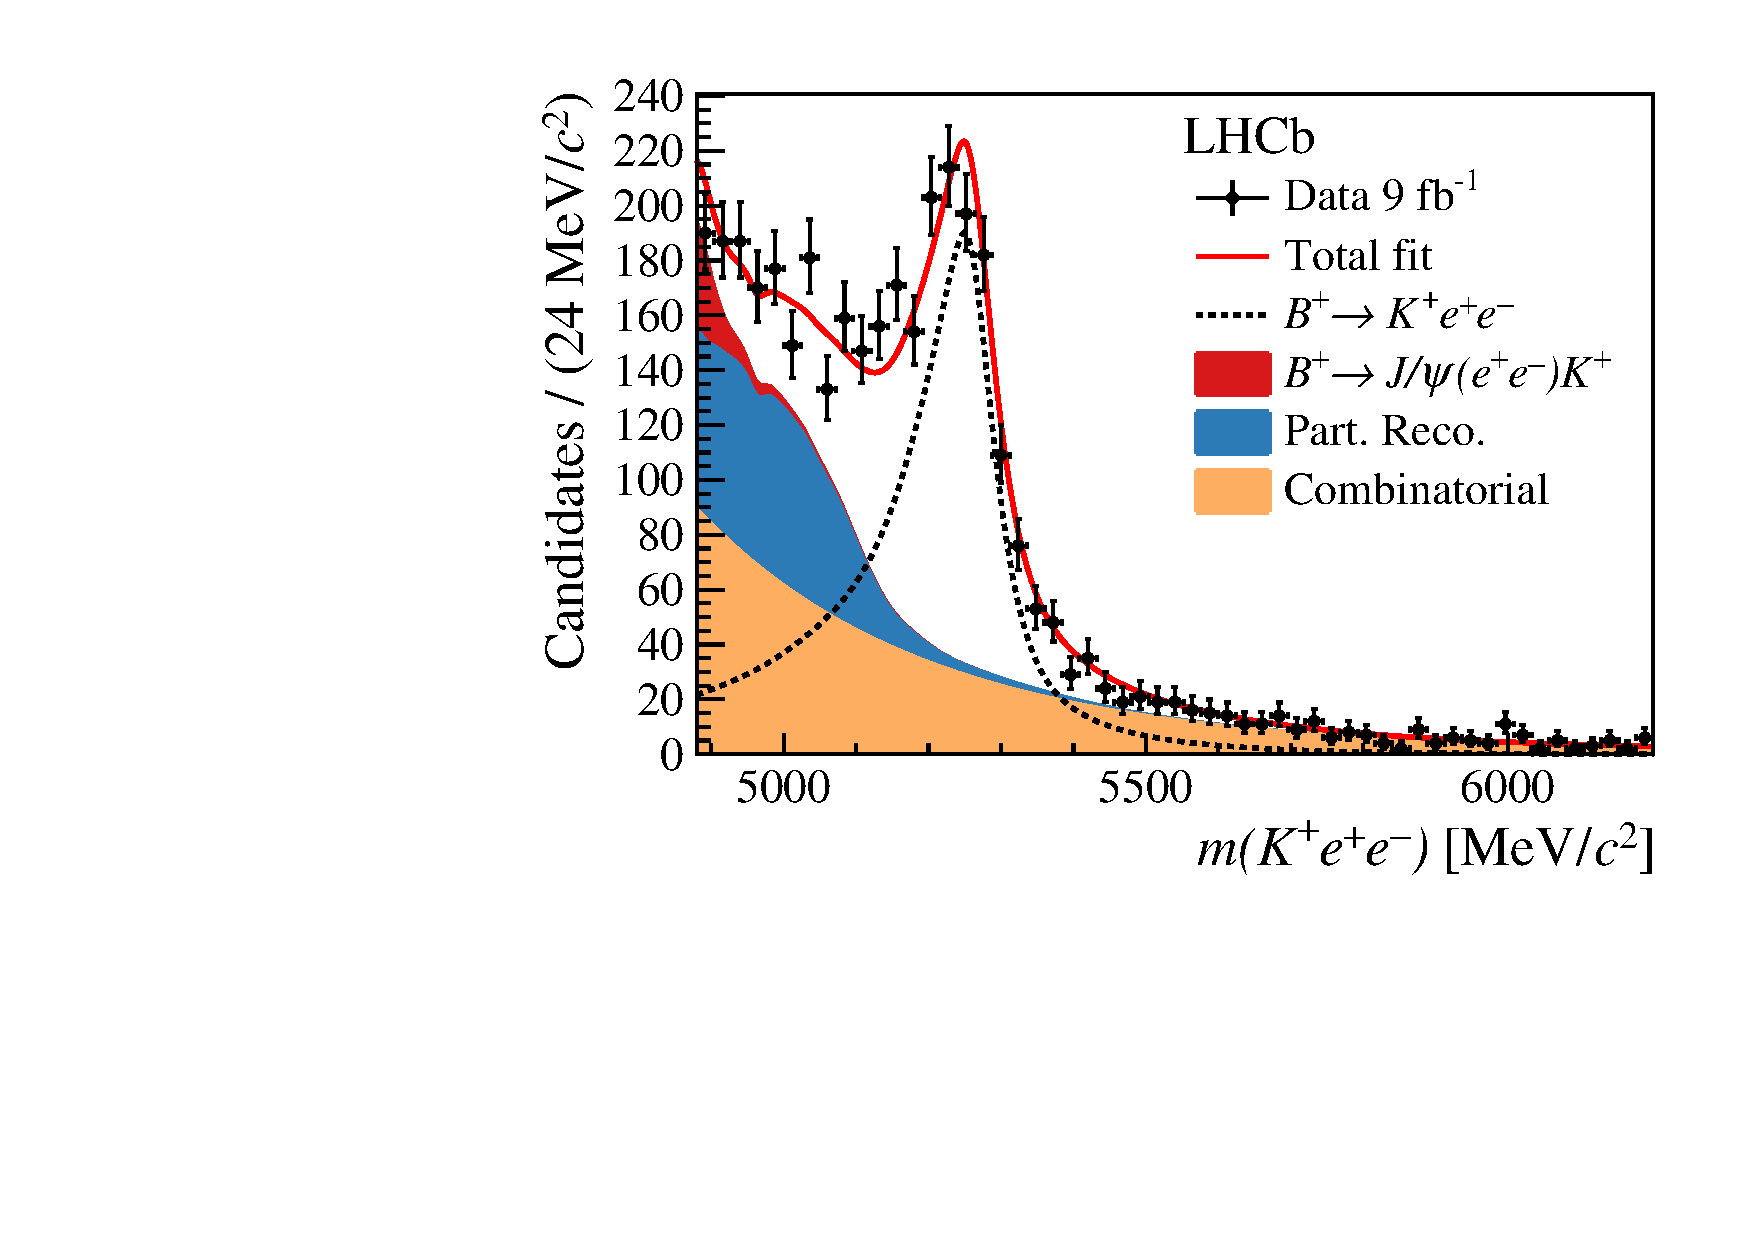
\includegraphics[width=0.45\textwidth]{figures/Fig2a.pdf}
    %plotKeeDataFitRunAllTrigAll.pdf}
    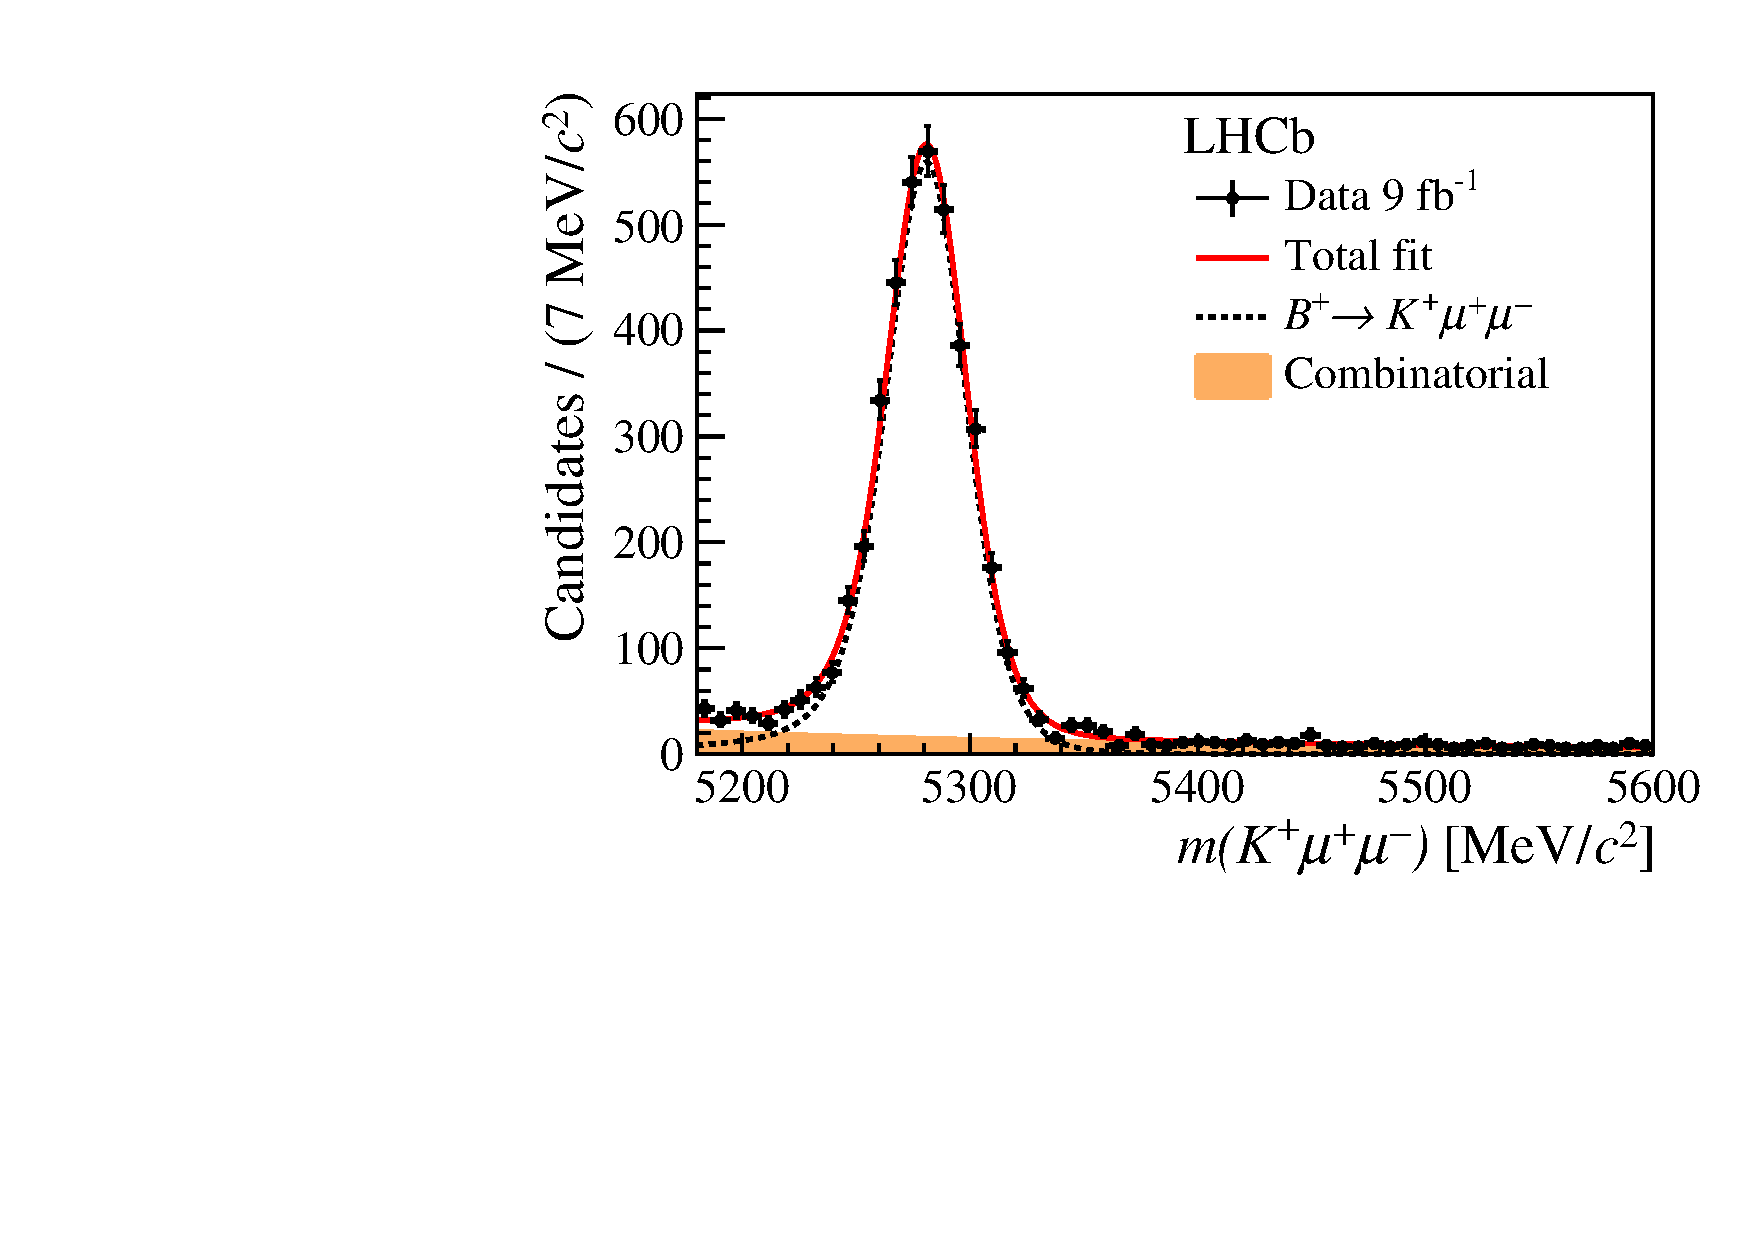
\includegraphics[width=0.45\textwidth]{figures/Fig2b.pdf}
    %plotKmumuDataFitRunAll.pdf}
    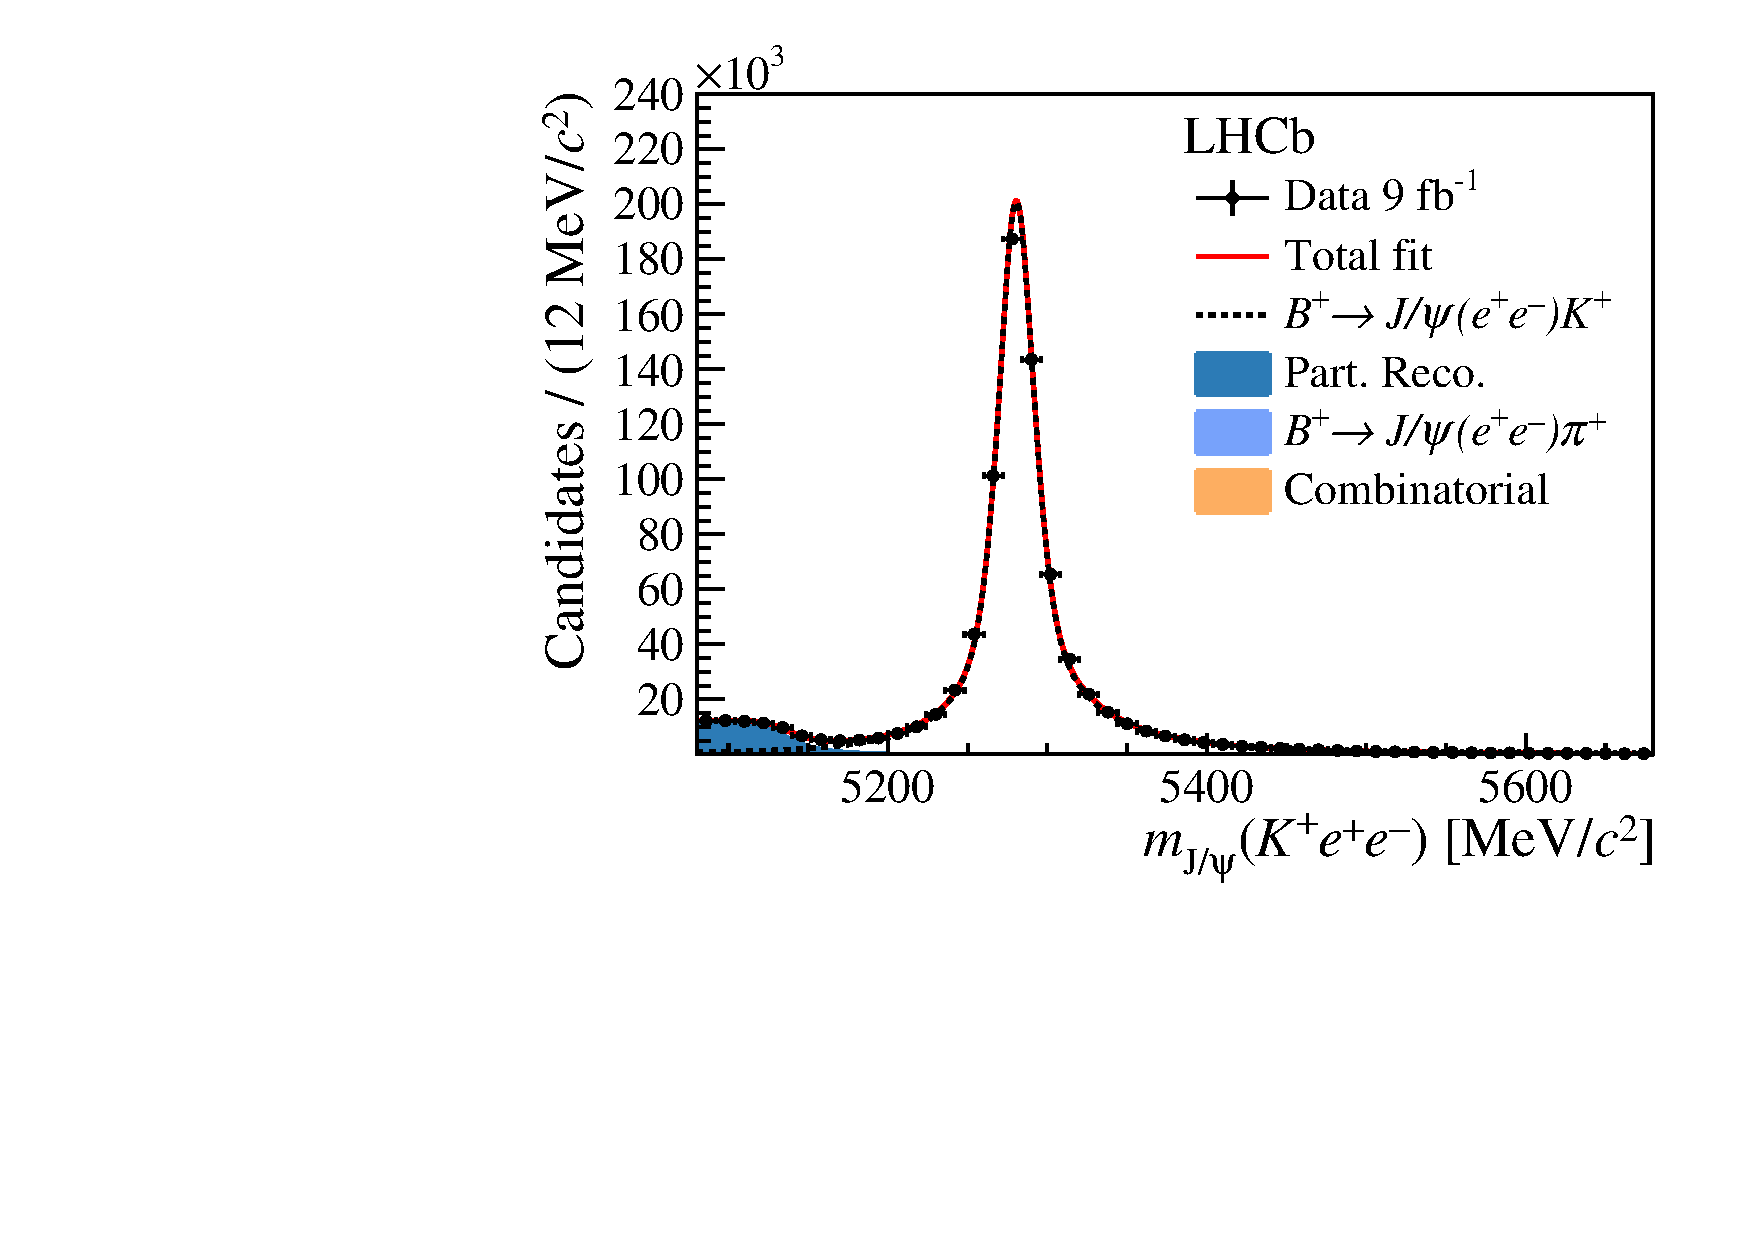
\includegraphics[width=0.45\textwidth]{figures/Fig2c.pdf}
    %plotKJpsieeDataFitTrig-1All.pdf}
    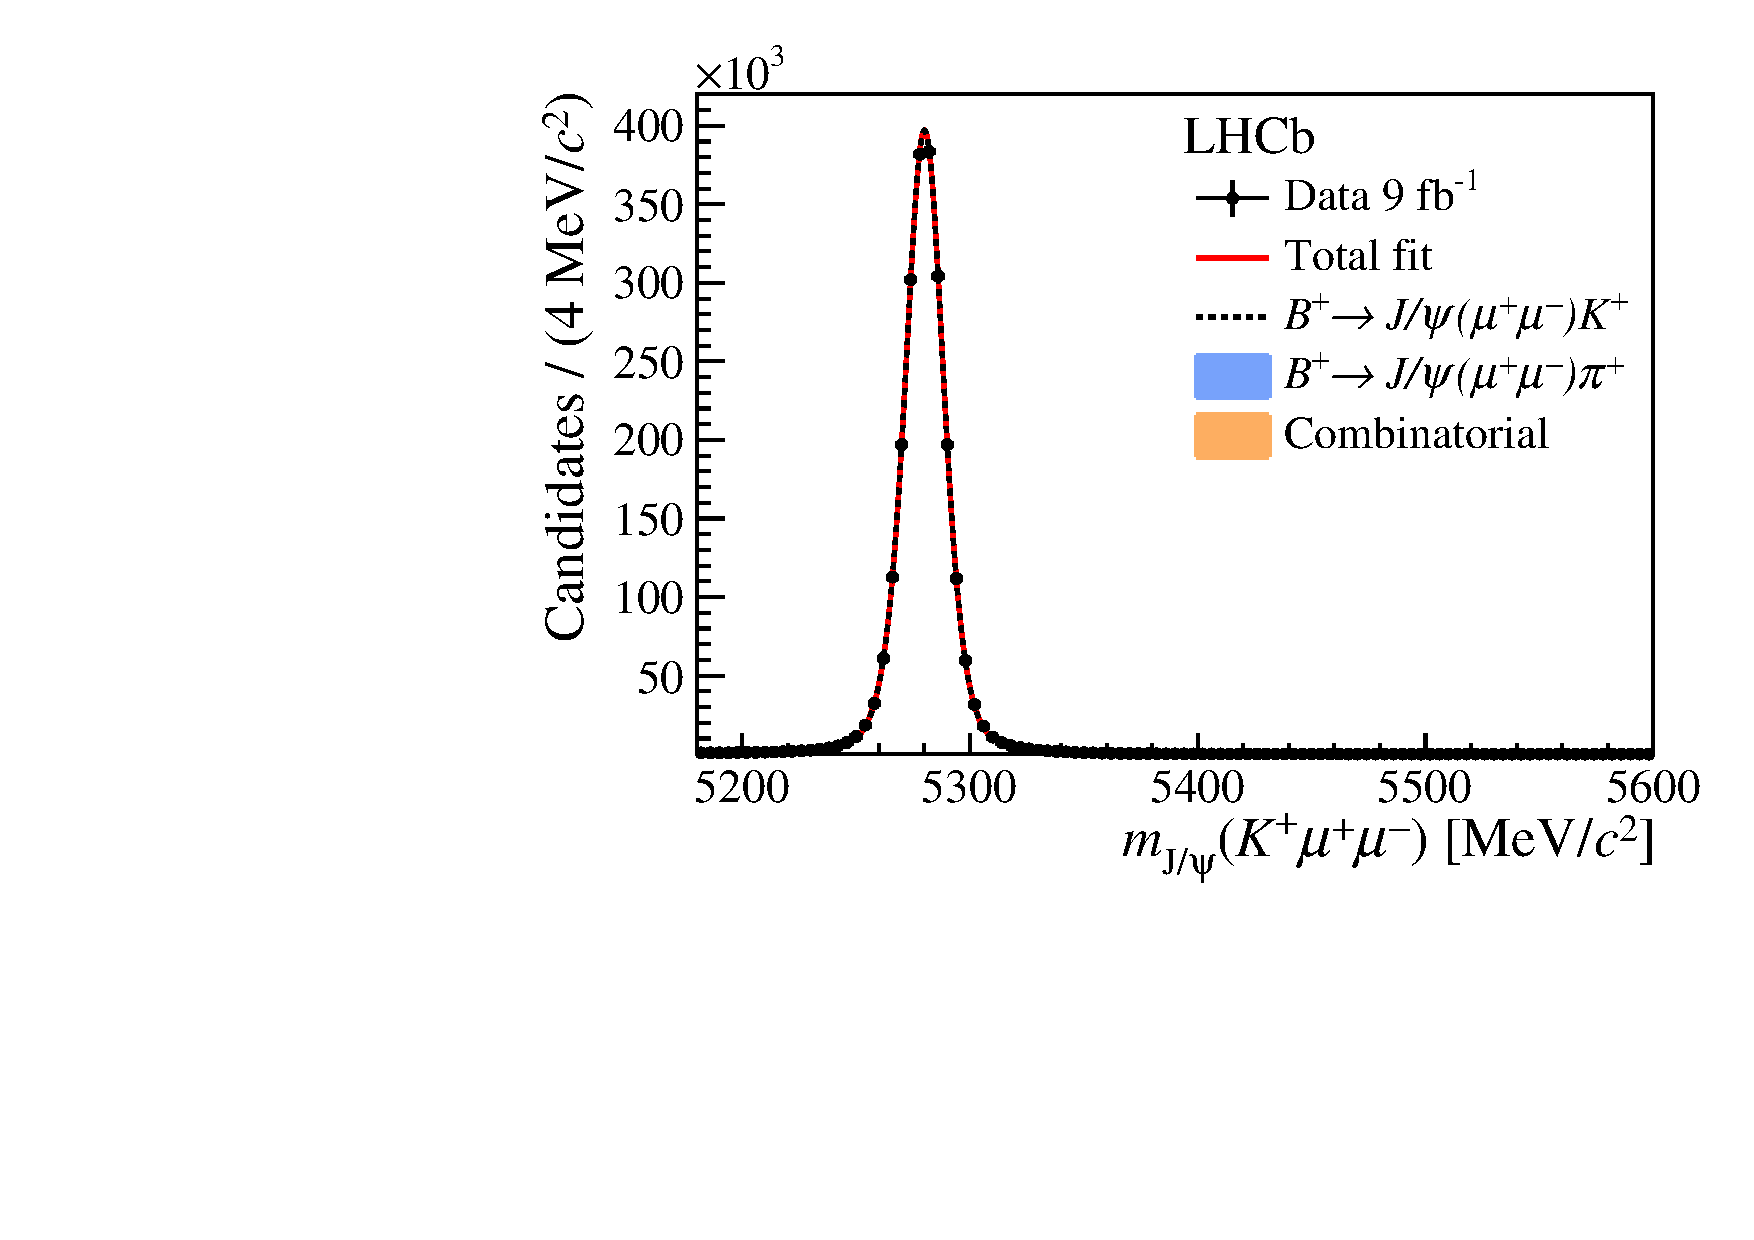
\includegraphics[width=0.45\textwidth]{figures/Fig2d.pdf}
    %plotKJpsimumuDataFitAll.pdf}
    \caption{Candidate invariant mass distributions. Distribution of the invariant mass \mKllgeneric for candidates with (left) electron and (right) muon pairs in the final state for the (top) nonresonant \BuKll signal channels and (bottom) resonant \BuJpsiKll decays. The fit projection is superimposed. In the resonant-mode distributions, some fit components are too small to be visible.
    }
    \label{fig:fits}
\end{figure}



After the application of the selection requirements, the resonant and nonresonant decays are clearly visible in the mass distributions (see Fig.~\ref{fig:fits}). The yields  in the two \BuKll and two \BuJpsiKll decay modes are determined by performing unbinned extended maximum-likelihood fits to these distributions (see Methods). 
For the nonresonant candidates, the \mKee and \mKmm distributions are fitted with a likelihood function that has the \BuKmm yield and \RK as fit parameters and the resonant decay-mode yields incorporated as Gaussian-constraint terms.
The resonant yields are determined from separate fits
to the mass, \mKllconst, formed by kinematically constraining the dilepton system to the known \jpsi mass~\cite{PDG2020} and thereby improving the mass resolution.



Simulated events are used to derive the two ratios of efficiencies needed to form \RK using Eq.~\eqref{eq:doubleratio}. Control channels are used to calibrate the simulation in order to correct for the imperfect modelling of the \Bu production kinematics and various aspects of the detector response. The overall effect of these corrections on the measured value of \RK is a relative shift of $(+3\pm1)\%$.
When compared with the 20\% shift that these corrections induce in the measurement of \rjpsi, this demonstrates the robustness of the double-ratio method in suppressing systematic biases that affect the resonant and nonresonant decay modes similarly.

The systematic uncertainty (see Methods) from the choice of signal and background mass-shape models in the fits is estimated by fitting pseudoexperiments with alternative models that still describe the data well. The effect on \RK is at the $1\%$ level. A  comparable uncertainty arises from the limited size of the calibration samples, with negligible contributions from the calibration of the \Bu production kinematics and modelling of the selection and particle-identification efficiencies. Systematic uncertainties that affect the ratios of efficiencies influence the measured value of \RK and are taken into account using constraints on the efficiency values. Correlations between different categories of selected events and data-taking periods are taken into account in these constraints. The combined statistical and systematic uncertainty is then determined by scanning the profile-likelihood and the statistical contribution to the uncertainty is isolated by repeating the scan with the efficiencies fixed to their fitted values.  

The determination of the \rjpsi ratio requires control of the relative selection efficiencies for the resonant electron and muon modes, and does not therefore benefit from the cancellation of systematic effects in the double ratio used to measure \RK. Given the scale of the corrections required, comparison of \rjpsi with unity is a stringent cross check of the experimental procedure. 
In addition, if the simulation is correctly calibrated, the measured \rjpsi value will not depend on any variable.
This ratio is therefore also computed as a function of different kinematic variables that are chosen to provide overlap with the spectra of the nonresonant decays. Although the range of \qsq differs between resonant and nonresonant decays, the efficiency depends on laboratory-frame variables such as the momenta of the final-state particles, or the opening angle between the two leptons, rather than directly on \qsq. A given set of values for the final-state particles' momenta and angles in the \Bp rest frame will result in a distribution of such values when transformed to the laboratory frame. As a result, there is significant overlap between the nonresonant and resonant samples in the relevant distributions, even if they are mutually exclusive as a function of \qsq. 

The value of \rjpsi is measured to be $0.981\pm0.020$, where the uncertainty includes both statistical and systematic effects.
The consistency of this ratio with unity demonstrates control of the efficiencies well in excess of that needed for the determination of \RK. 
In the measurement of the \rjpsi ratio, the systematic uncertainty is dominated by the imperfect modelling of the \Bu production kinematics and the modelling of selection requirements, which have a negligible impact on the \RK measurement.
No significant trend is observed in the differential determination of \rjpsi as a function of any considered variable. An example distribution, with \rjpsi determined as a function of \Bp momentum component transverse to the beam direction, \pt, is shown in Fig.~\ref{fig:rjpsi_differential}. Assuming the observed \rjpsi variation in such distributions reflects genuine mismodelling of the efficiencies, rather than statistical fluctuations, and taking into account the spectrum of the relevant variables in the nonresonant decay modes, a total shift on \RK is computed for each of the variables examined. In each case, the resulting variation is within the estimated systematic uncertainty on \RK. Similarly, double differential
computations of the \rjpsi ratio also do not show any trend and are consistent with the systematic uncertainties assigned on the \RK measurement.

\begin{figure}[!b]
   \begin{center}

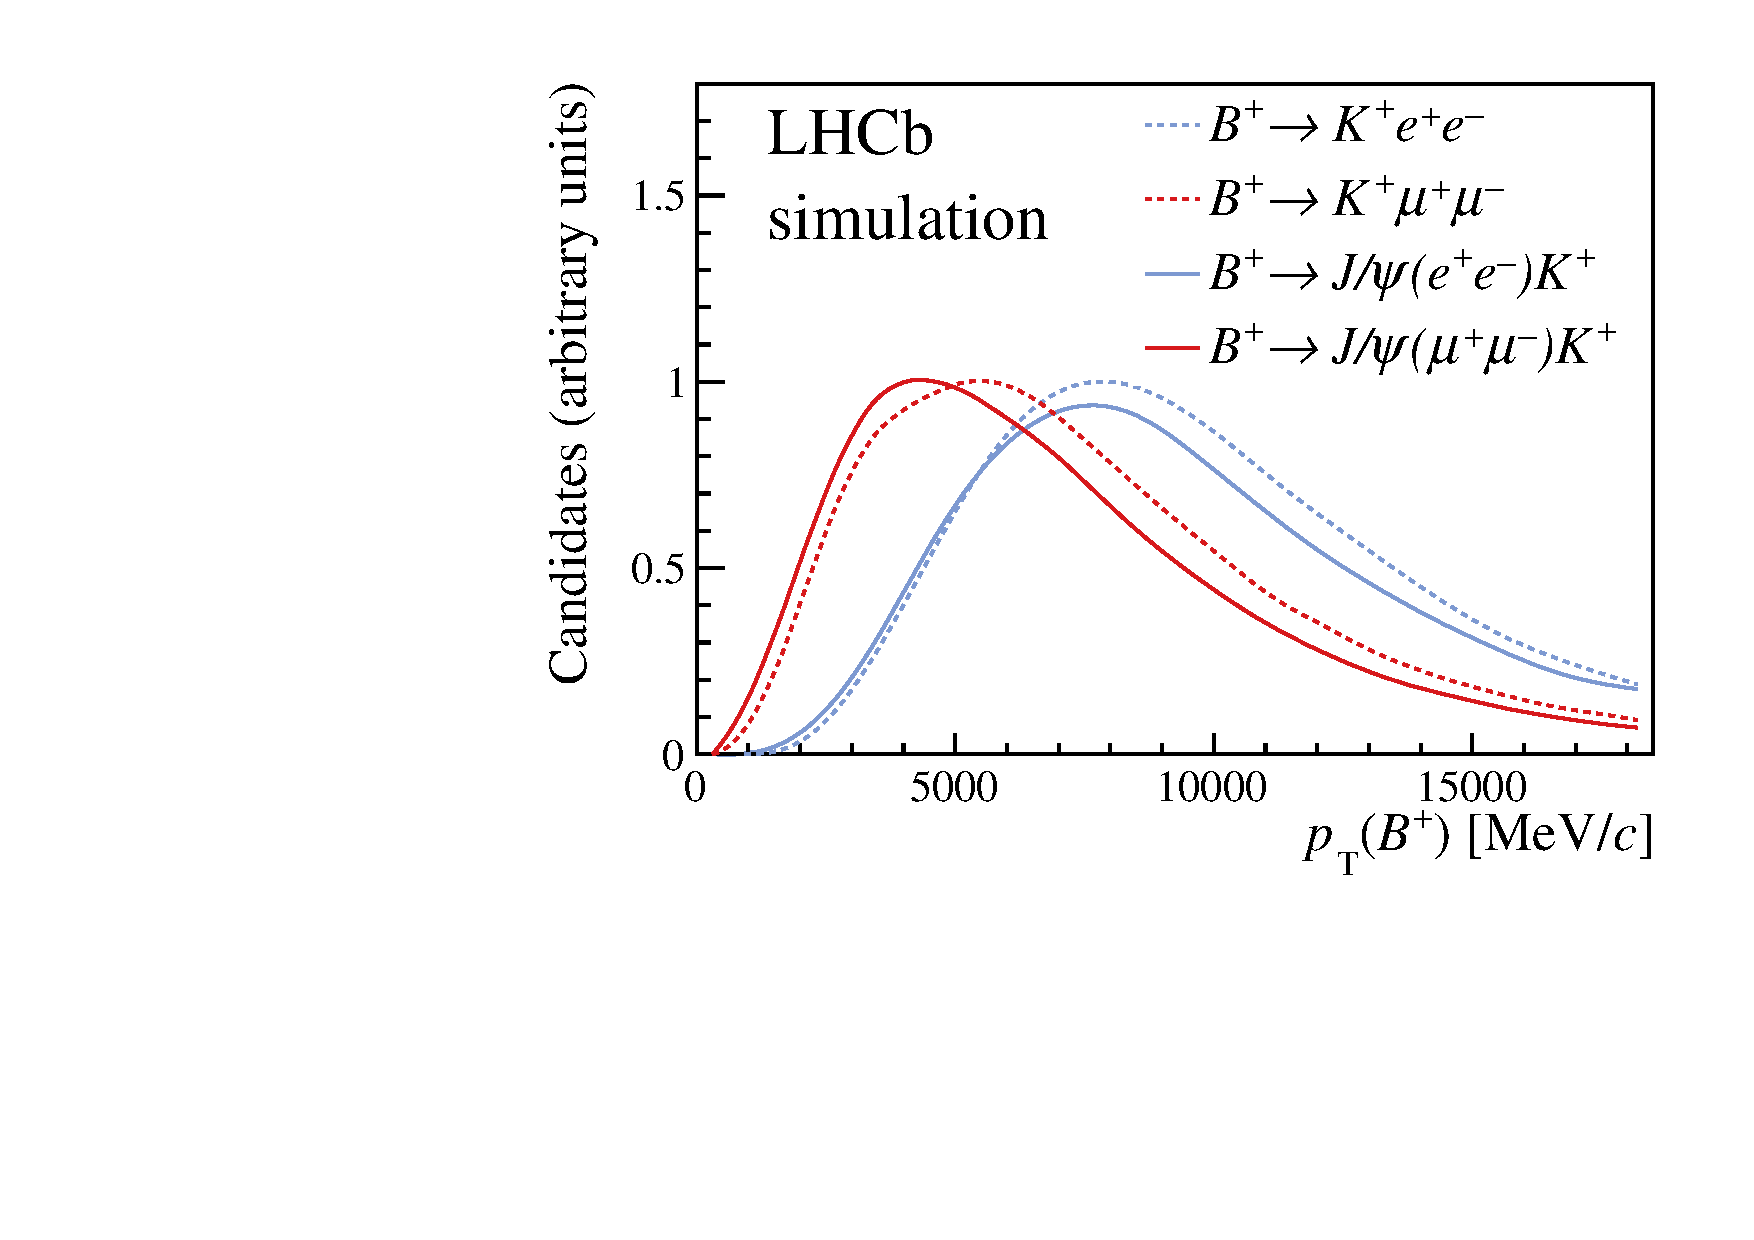
\includegraphics[width=0.45\linewidth,trim={0 0 0 0.5cm}, clip]{figures/Fig3a.pdf}
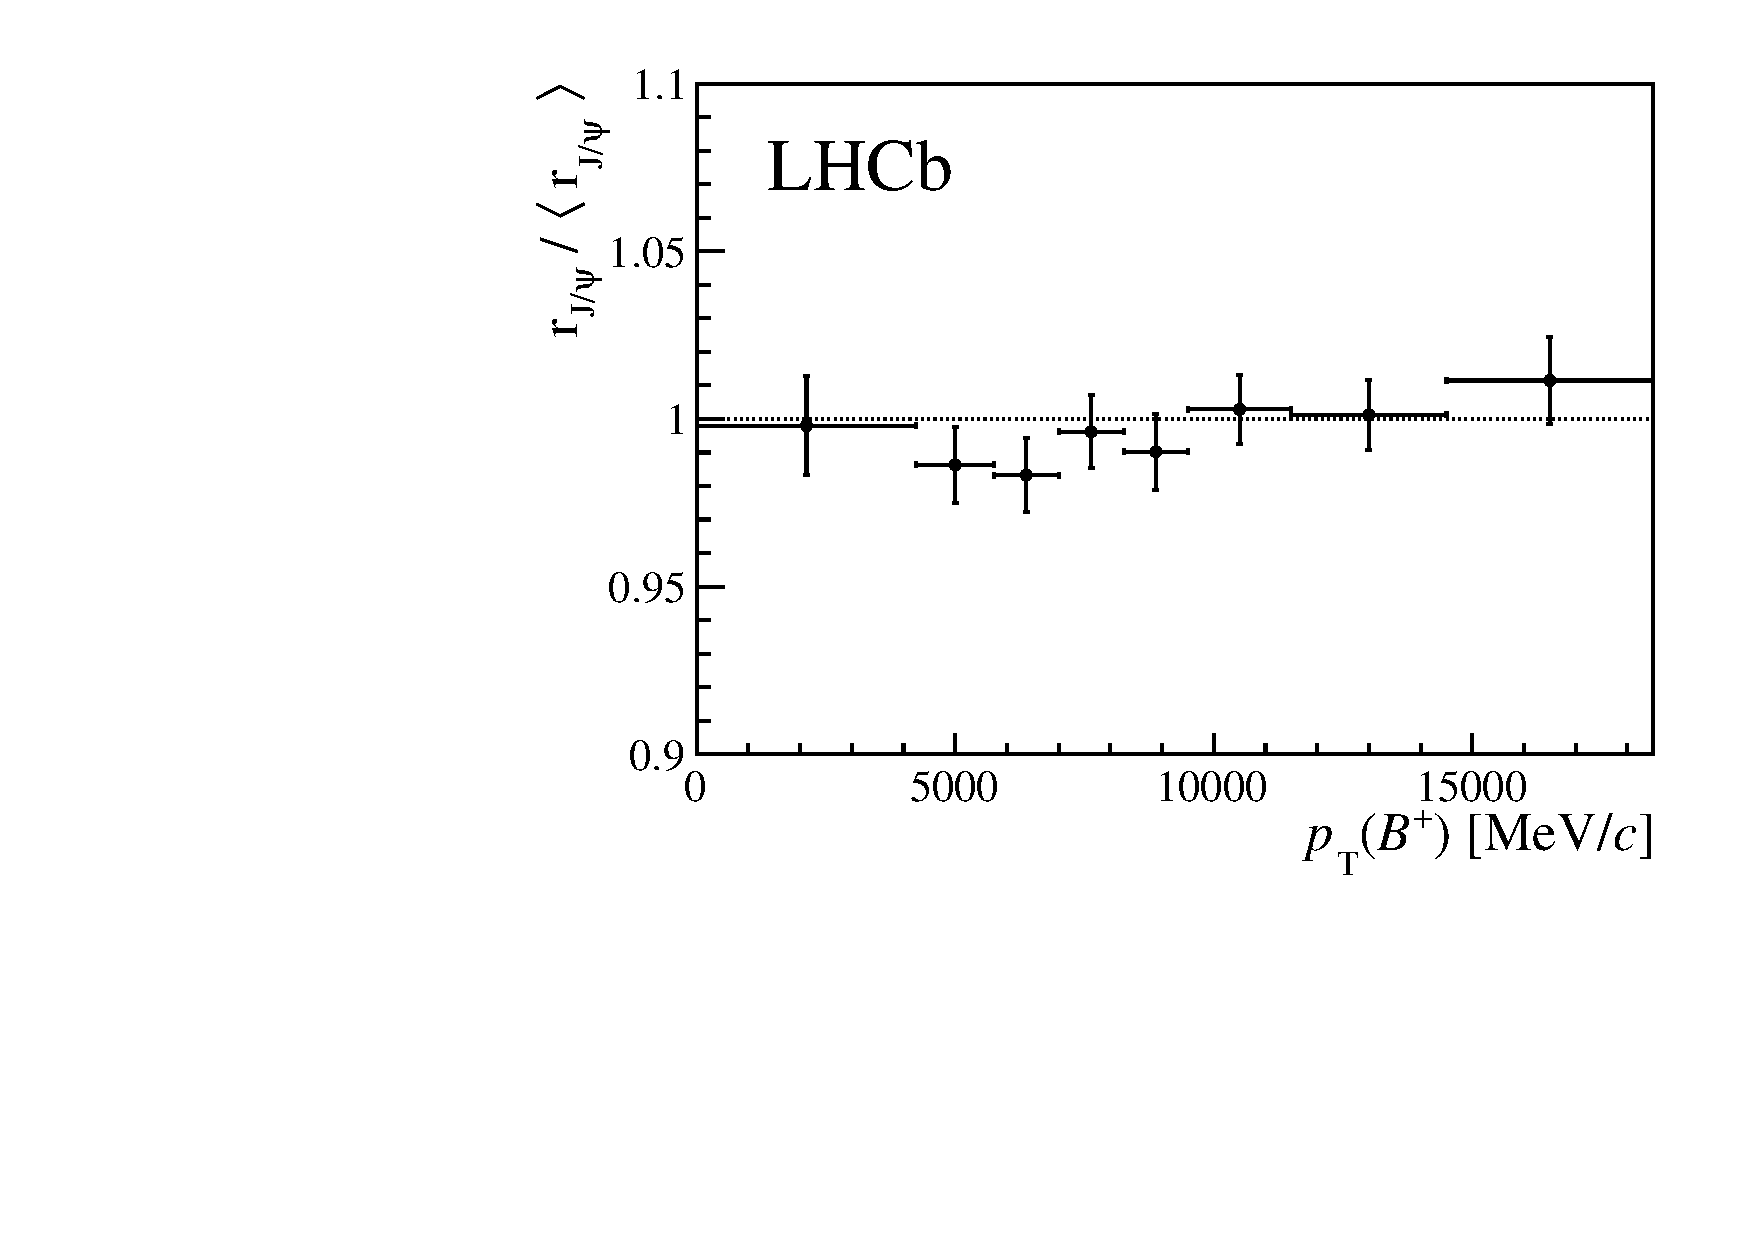
\includegraphics[width=0.45\linewidth,trim={0 0.15cm 0 0}, clip]{figures/Fig3b.pdf}
      \end{center}
      \caption{Differential \rjpsi measurement. The 
      distributions of (left) the \Bp transverse momentum, \pt, and (right) the ratio \rjpsi relative to its average value $\left< \rjpsi \right>$ as a function of \pt. The distribution from the \BuJpsiK decays is similar to that of the corresponding \BuKll decays such that the measurement of \rjpsi tests the kinematic region relevant for the \RK measurement. The lack of any dependence of the value of $\rjpsi/\left< \rjpsi \right>$ as a function of \Bp $p_{\mathrm T}$ demonstrates control of the efficiencies.}
    \label{fig:rjpsi_differential}
\end{figure}

In addition to \BuJpsiK decays, 
clear signals are observed from \BuPsiK decays. 
The double ratio of branching fractions, \RPsitwos, defined by
\begin{equation}
\label{eq:RPsitwos}
\RPsitwos  =
{\frac{\BR(\BuPsiKmm)}{\BR(\BuJpsiKmm)}} \bigg{/} {\frac{\BR(\BuPsiKee)}{\BR(\BuJpsiKee)}}  \,,
\end{equation}
\noindent provides an independent validation of the double-ratio analysis procedure and further tests the control of the efficiencies. 
This double ratio is expected to be close to unity~\cite{PDG2020}
and is determined to be $0.997\pm 0.011$, where the uncertainty includes both statistical and systematic effects.
This can be interpreted as a world-leading test of lepton flavour universality in $\psi(2S) \rightarrow \ell^+\ell^-$ decays.

The fit projections for the \mKll and \mKllconst distributions are shown in Fig.~\ref{fig:fits}. The fit is of good quality and the value of \RK is measured to be
\begin{displaymath}
\RK (1.1 < \qsq < 6.0 \gevgevcccc) = \RKvalue\,,
\end{displaymath}
\noindent where the first uncertainty is statistical and the second systematic. Combining the uncertainties gives $\RK=\RKvalueComb$.
This is the most precise measurement to date and is consistent with the SM expectation, \mbox{$1.00 \pm 0.01$}~\cite{Descotes-Genon:2015uva,Bobeth:2007,Bordone:2016gaq,EOS,Straub:2018kue}, at the level of 0.10\% (\significance~standard deviations), giving evidence for the violation of lepton universality in these decays.
The value of \RK is found to be consistent in subsets of the data divided on the basis of data-taking period, selection category and magnet polarity (see Methods).
The profile-likelihood is given in Methods. A comparison with previous measurements is shown in Fig.~\ref{fig:RKresult}.

The $3850\pm 70$ \BuKmm decay candidates that are observed are used to compute the \BuKmm  branching fraction as a function of \qsq. The results are consistent between the different data-taking periods and with previous \lhcb measurements~\cite{LHCb-PAPER-2014-006}.
The \BuKee branching fraction is determined by combining the value of \RK with the value of $\deriv\BR(\BuKmm)/\deriv\qsq$ in the region $(1.1 < \qsq < 6.0 \gevgevcccc)$~\cite{LHCb-PAPER-2014-006}, taking into account correlated systematic uncertainties. This gives
\begin{displaymath}
\frac{\deriv\BR(\BuKee)}{\deriv\qsq}(1.1 < \qsq < 6.0 \gevgevcccc)  = (28.6\,^{+\, 1.5}_{-\, 1.4} \,\pm 1.3)\times 10^{-9}\,c^4\kern -0.1em/\kern -0.15em\gev^2\,.
\end{displaymath}
\noindent The limited knowledge of the \BuJpsiK branching fraction~\cite{PDG2020} gives rise to the dominant systematic uncertainty. This is the most precise measurement of this quantity to date and, given the large theoretical uncertainty on the predictions~\cite{Khodjamirian:2017fxg,Straub:2018kue}, is consistent with the SM.


A breaking of lepton universality would require an extension of the gauge structure of the SM that gives rise to the known fundamental forces. It would therefore constitute a significant evolution in our understanding and would challenge an inference based on a wealth of experimental data in other processes. Confirmation of any beyond the SM effect will clearly require independent evidence from a wide range of sources.

\begin{figure}[!t]
    \centering
    %RK2021_column
    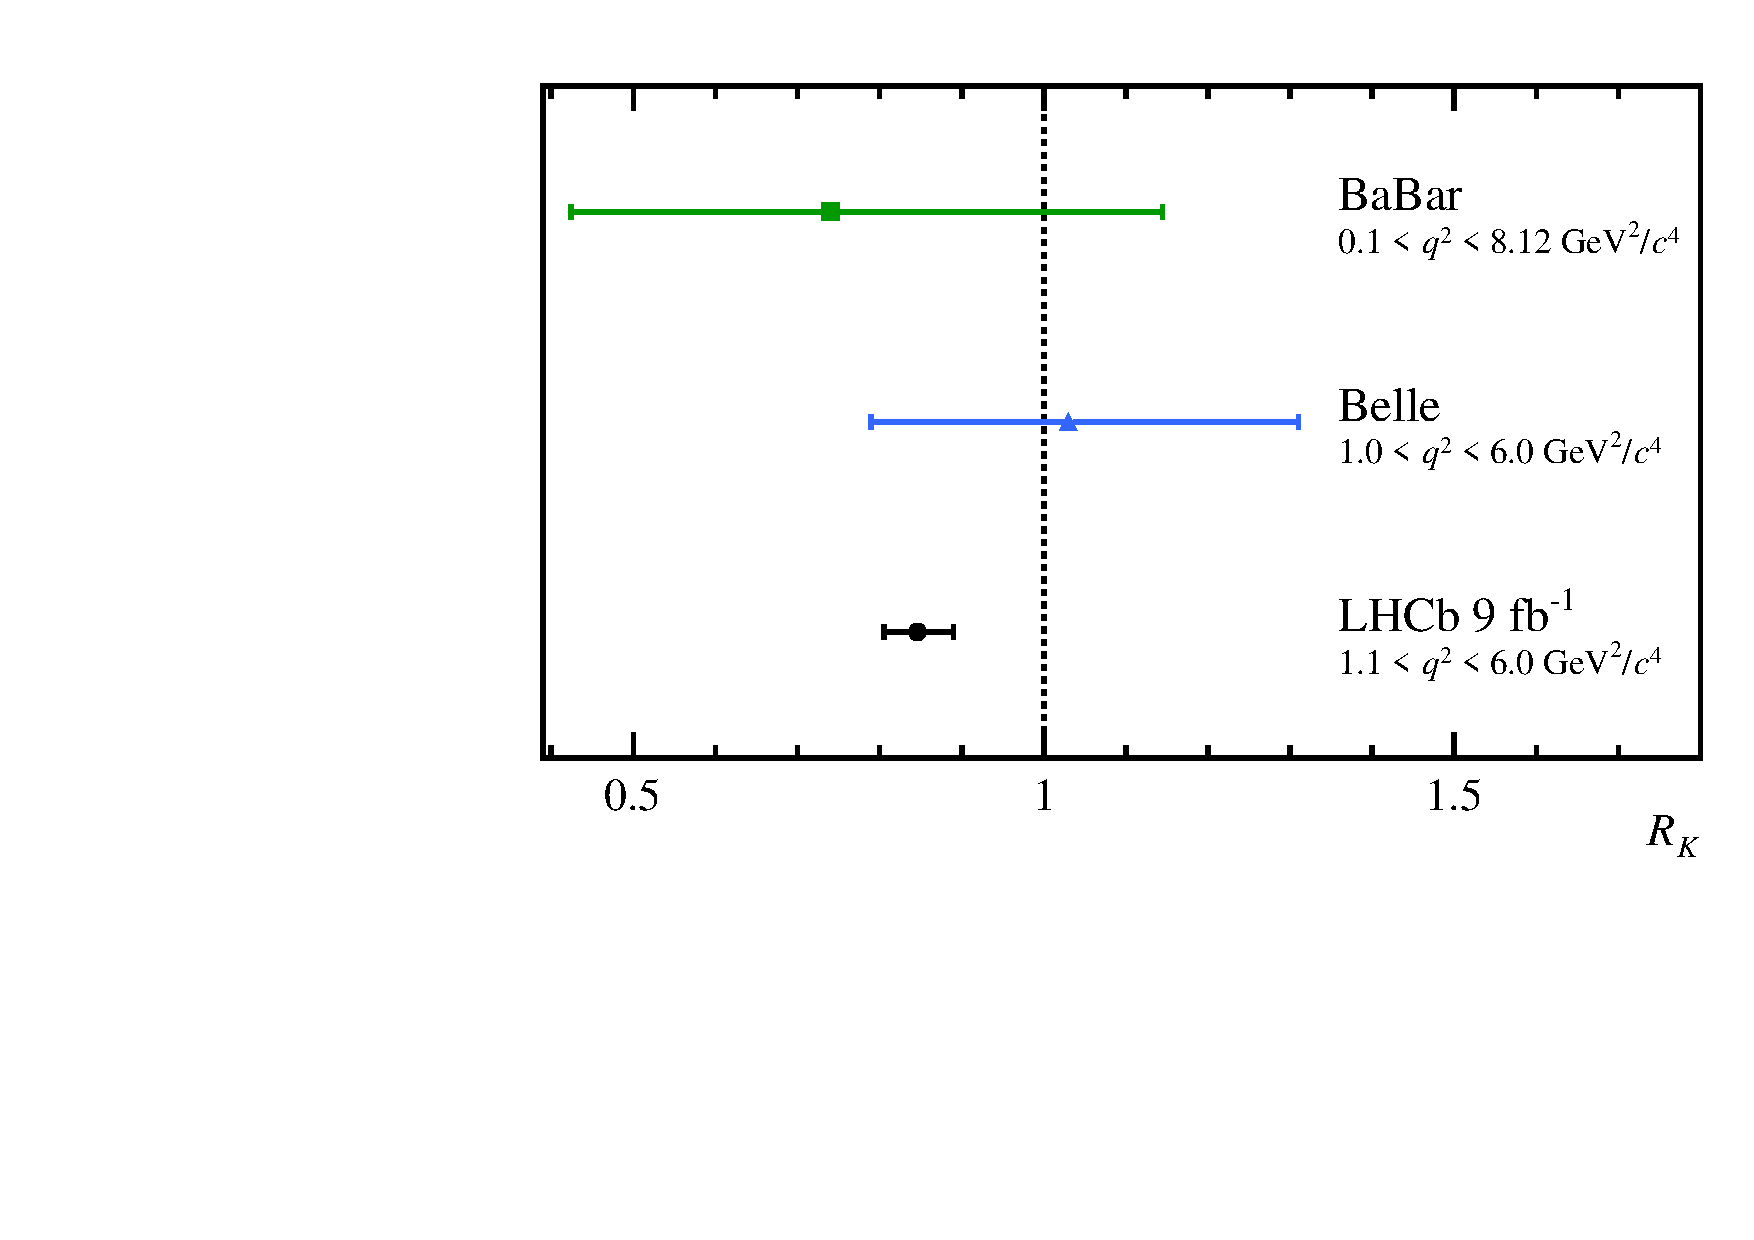
\includegraphics[width=0.7\textwidth]{figures/Fig4.pdf} 
    \caption{Comparison between \RK measurements. 
    In addition to the LHCb result, the measurements by the BaBar~\cite{RKbabar} and Belle~\cite{RKbelle} collaborations, which combine \BuKll and \BdKSll decays, are also shown.
    }
    \label{fig:RKresult}
\end{figure}

Measurements of other $R_H$ observables with the full LHCb data set will provide further information on the quark-level processes measured. 
In addition to affecting the decay rates, new physics can also alter how the decay products are distributed in phase space. 
An angular analysis of the electron mode, where SM-like behaviour might be expected in the light of the present results and those from \btosmumubar decays, would allow the formation of ratios between observable quantities other than branching fractions, enabling further precise tests of lepton universality~\cite{Altmannshofer:2015mqa,Capdevila:2016ivx,Wehle:2016yoi,Geng:2017svp,Serra:2016ivr}. The hierarchical effect needed to explain the existing \bsllbar and \btoclnubar data, with the largest effects observed in tau modes, then muon modes, and little or no effects in electron modes, suggests that studies of \btostautaubar transitions are also of great interest~\cite{LHCb-PAPER-2017-003, TheBaBar:2016xwe}. There are excellent prospects for all of the above and further measurements with the much larger samples that will be collected with the upgraded LHCb detector from 2022 and, in the longer term, with the LHCb Upgrade~II~\cite{LHCb-PII-Physics}. Other experiments should also be able to determine $R_H$ ratios, with the Belle II experiment in particular expected to have competitive sensitivity~\cite{Kou:2018nap}.

In summary, in the dilepton mass-squared region $1.1 < \qsq < 6.0 \gevgevcccc$, the ratio of branching fractions for \BuKmm and \BuKee decays is measured to be $\RK=\RKvalueComb$. 
This is the most precise measurement of this ratio to date and is compatible with the SM prediction with a p-value of 0.10\%. The significance of this discrepancy is \significance standard deviations, giving evidence for the violation of lepton universality in these decays.